%
% File: chap03.tex
% Author: Hongliang Zhong
% Description: Introduction chapter where the biology goes.
%
\let\textcircled=\pgftextcircled
\chapter{Bandit with side information}
\label{chap:BF}

 \initial{C}ontextual Bandit, where the Bandit problem with side information has been introduced in Section~\ref{subsec:contextual}. Since it is closely related to work on supervised learning and reinforcement learning, it is usually applied to solve the problem of supervised learning with partial feedback. The classification with partial feedback is a novel and influential problem. It can be traced back to online classification with full feedback and multi-armed bandit learning. This Classification can be considered as a Multi-Armed Bandit problem with side information. Langford \cite{langford2008epoch} extended the Multi-Armed setting to the case where some side information is provided. But, the setting has a high level of abstraction and its application to the classification bandit learning is not straightforward. 
 
In this chapter, we restate the setting in Supervised learning with partial feedback under the frame of Contextual Bandit (in this chapter, it will be called Bandit Feedback), and recall some outstanding researches and contributions. 
At first, we formally re-introduce some notations in the modeling of Bandit Feedback. Just as what we have previously presented, the problem of Bandit Feedback is composed by two parts: supervised classification learning and partial feedback. 
For the side of the classification learning, we will focuse on introducing some supervised classification algorithms in the-state-of-art. From other side, we present some important algorithms working with Bandit Feedback, most of them are based on the supervised learning algorithm combining some bandit strategies. 
After completing the description of the classification with Bandit Feedback, we repose a novel problem, the Multi-Labels classification working with partial feedback. Then, we provide some analysis and some effective algorithm to this issue. 
Finally, to evaluate the quality of those algorithms, we take some experimentation on comparing them with classical datasets and analyze their respective features and benefits.


\
\
\
\
\
\

%=========================================================

%=======
\section{Bandit feedback in Multi-class Classification}
\label{sec:BF01}
Classification is a fundamental task of machine learning, and is by now well understood in its basic variants. Unlike the well-studied supervised learning setting, many recent applications (such as recommender system, ad selection,etc) can not work under the frame of  the supervised learning with side information. In this section, we introduce this kind problem: Online Classification with \textbf{Bandit Feedback}.

Online classification with bandit feedback, is a bandit variant of the online classification protocol, where the goal is to sequentially learn a mapping from the context space $\inputS \subseteq\Rd$ to the label space $\outputS=\left\lbrace 1,\dots,K\right\rbrace$, with $K\geq 2$. In this protocol, forecaster keeps  classifiers parameterized $w=(w_1,w_2,\dots,w_K)$ from the hypothesis space $\mathscr{W} \subseteq \mathbb{R}^{K \times d} $. At each steps $t = 1,2,\dots,T$, the side information $x_t \in \inputS$ is sampled as i.i.d., then forecaster predicts the label $\hy$, by the linear hypothesis $w$:
\begin{equation}
\label{equa:prediction}
\hy = \underset{k\in\{1,\dots,K\}}{\text{argmax}} <w_k,x_t>
\end{equation}

In the standard online protocol, forecaster observes the true label $y_t$ associated with $x_t$ after each prediction and uses this full information to adjust the classifier $w_t$. However, in the bandit version, forecaster only observes an indicator $\1(\hy = y_t)$, that is , whether the prediction at time $t$ is correct or not. We denote the cumulative loss of supervised learning as following:
\begin{equation}
\label{equa:cumuloss}
L = \sum_{t=1}^T l \left(w_t; (\instance,\hy)\right)
\end{equation}
And the one with Bandit Feedback is defined as below:
\begin{equation}
\label{equa:cumulossBF}
L_{BF} = \sum_{t=1}^T l_{BF} \left(w_t; (\xt,\1(\hy=y_t)\right)
\end{equation}

\subsection{Multiclass Classification}
\label{subsec:multiclass}

Multiclass Classification is a problem of classifying the samples into several different classes and online learning is performed as a sequence of trials experiment. To solve this problem, the algorithms are aiming at learning a predictor $h: \mathscr{X} \rightarrow \mathscr{Y}$, which maps the instances to the classes space. The simplest approach to tackle multiclass prediction problem is by reduction from multiclass classification to binary classification. That is the methods we often mention: One-versus-All and All-versus-All. See Figure~\ref{pig:multiclass0}, there are some points classified into three classes (classified as their colors), by the method One vs All, it's necessary to find three binary classifiers who can only identify one class see Figure~\ref{pig:multiclass123}. Crammer has introduced several additive and multiplicative algorithms in \cite{crammer2003ultraconservative}, where Perceptron \cite{rosenblatt1958perceptron} and Winnow \cite{littlestone1988learning} are two such important algorithms. Much analysis has been done, Kivinen and Warmuth developed potential functions that can be used to analyze different online algorithm \cite{kivinen1995additive}. 

\begin{figure}[!h]
\vspace{.2in}
\centering{
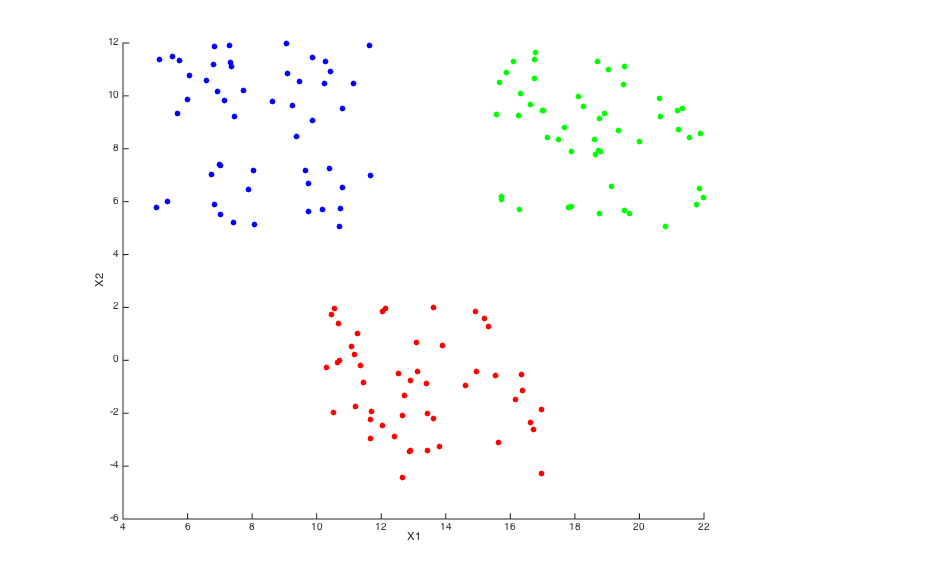
\includegraphics[scale = 0.5]{chapters/chapter03/fig03/mc/originalml.png}}
\caption{Multiclass task}
\label{pig:multiclass0}
\end{figure}

\begin{figure}[!h]
\vspace{.2in}
\centerline{
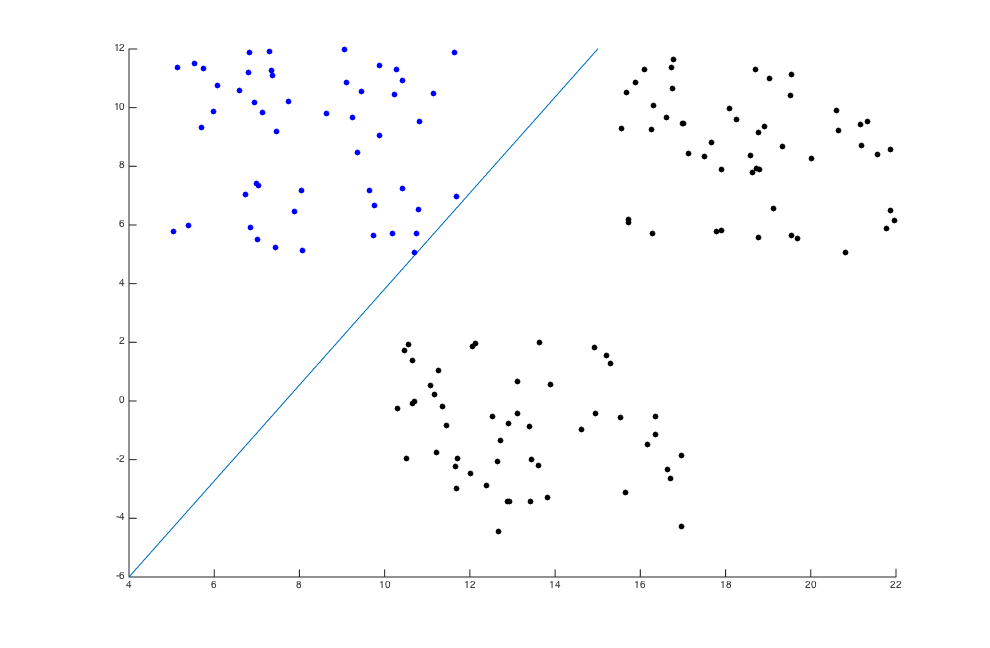
\includegraphics[width=0.6\linewidth]{chapters/chapter03/fig03/mc/class1.png}}
\centerline{
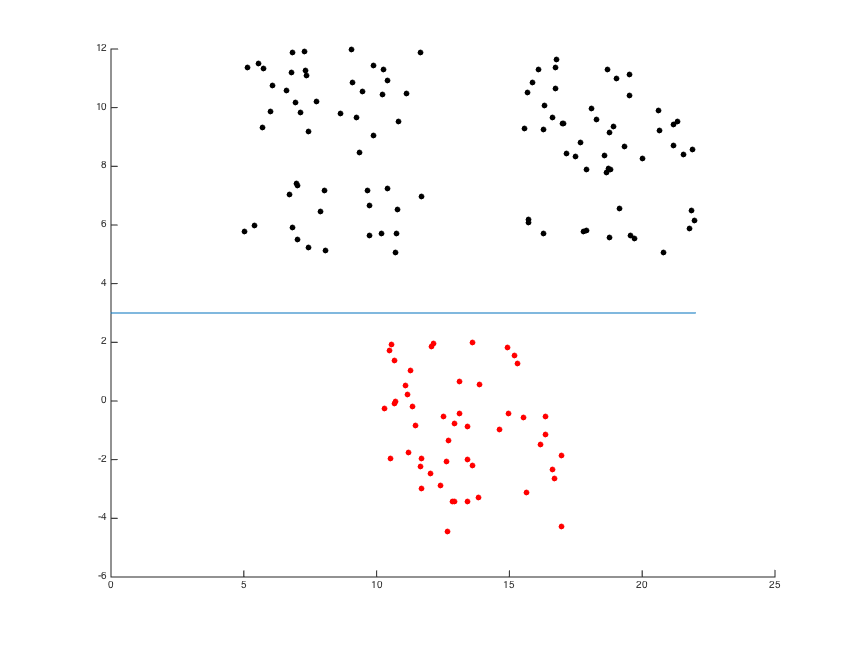
\includegraphics[width=0.6\linewidth]{chapters/chapter03/fig03/mc/class2.png}}
\centerline{
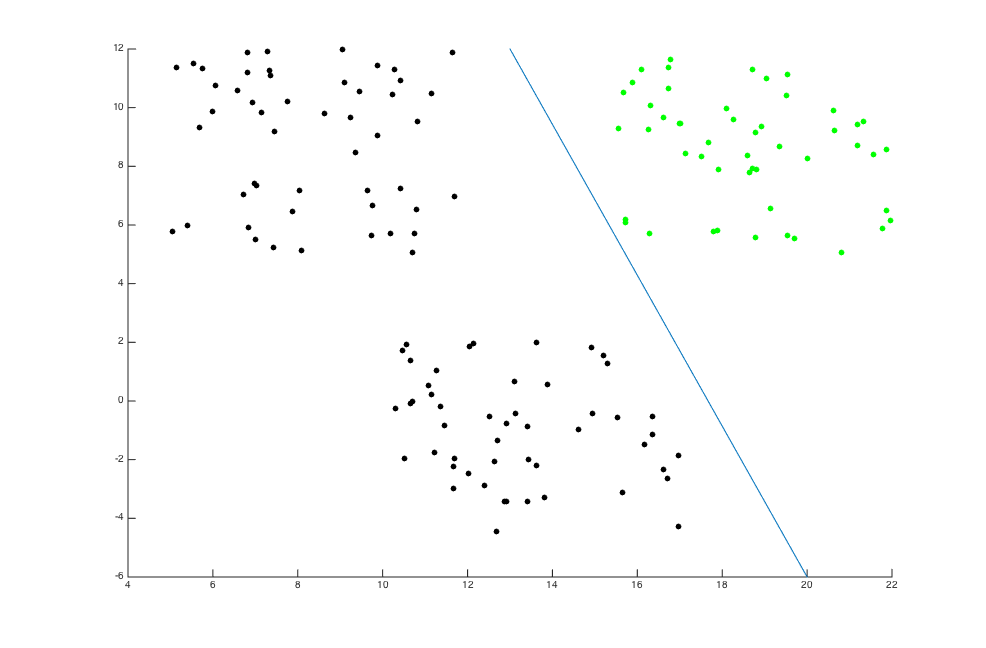
\includegraphics[width=0.6\linewidth]{chapters/chapter03/fig03/mc/class3.png}}
\caption{Reduction from multiclass classification to binary classification (One vs All)} 
\label{pig:multiclass123}
\end{figure}

For the process of multiclass classification online learning, at trial $t$, the algorithm firstly samples an instance $x_t \in \inputS\subseteq \Rd$ and classifies it into the set of all possible labels constitutes a finite set denoted by $\outputS$. Mostly, the algorithms of online classification assume that $\outputS$ is known in advance. We denote the set of unique labels observed on rounds from $1$ to $t-1$ by $Y_t$ ( In general, this set is known in advance and non-changeable during all rounds, so it could be simplified by $Y$). After predicted the label $\hy$ by the algorithm of online learning, the true class $y_t\in Y_t$ is revealed. Sometimes, the prediction $\hy$ is different to the true label $y_t$, in that case, it makes an incorrect prediction. To evaluate the accuracy or quality of classifiers, the prediction mistakes (denoted as $M$), regret (or instantaneous loss, as $l$) or cumulative regret (denoted as $R$ or $L$) come into being. To be computed on each round, specially when $\hy \neq y_t$.

The goal of all classification algorithms, is to minimize the total number of prediction mistakes or cumulative regret. To achieve this goal, the algorithms should update the classifiers by supervised learning mechanism at the end of each trial. 

Here, we make some definitions:  the feature vector representation $\pxy$ induced by the instance label pair $(\mathbf{x},y)$. Here, $\pxy$ is a $K\times d$ matrix which is composed of $K$ blocks of feature size $d$. All blocks but the $y$'th block of $\pxy$ are set to be the zero vector while the $y$'th blocks is set to be $\mathbf{x}$. Applying a single prototype multi-class algorithm to this problem produces a hypothesis $w \in \mathbb{R}^{K\times d}$ from $\mathscr{W}$ on every online round. Analogous to the construction of $\pxy$, $w$ is composed of $K$ blocks of size $d$ and denote block $r$ by $w_r$. By construction, we get that $<w \cdot \Phi(x_t,r) >= <w_r, x_t>$. Recall the hinge loss in binary classification, it's defined to be $[1-y_t<w,\xt>]_+$, where $[a]_+$ means $\text{max}(a,0)$. The hinge loss in the multiclass frame as follows:
\begin{equation}
\label{equa:hingelossML}
l(w_t;(\xt,y_t,\hy)) = [1+ <w_t, \Phi(\xt,\hy)> - <w_t, \Phi(\xt,y_t)>]_+
\end{equation}
After introduce the principal multiclass definitions, in the following of this section, we study some approaches for learning multiclass classifiers. Most of them are linear multiclass predictors. 

\vspace{3ex}
\textbf{Perceptron} was proposed by F. Rosenblatt \cite{rosenblatt1958perceptron}. It is a general computational model with some numerical weights. By Minsky and Papert \cite{minsky1987perceptrons}, it was refined and perfected in 1960s.  For the simplest binary model, the input space $\mathscr{X}\subseteq \mathbb{R}^d$ can be separated into two sets $P$ and $N$. The algorithm Perceptron is to look for a weight vector $w\in \mathbb{R}$ with a product function $h$, where $h(x_t) = <w,x_t> \in \mathbb{R}$. If the $P$ and $N$ are linear separated, the ideal weighted vector be assumed that all points of $P$ holds the product $h(x_P) > 0$ and all points of $N$ holds $h(x_N) < 0$. 

Generally, it initiates to choose the weight vector $w_0$ randomly. For the binary state, if the instance on round $t^{th}$ $x_t$ belongs to the set $P$,  $y_t$ the class of instance $x_t$ is $+1$, else $y_t$ equals to $-1$. Then, $y_t\cdot h(x_t) > 0$, it means the weight vector make a good prediction, and continue to predict a new instance; from the opposite direction, when it predicts wrong, the value of product $y_t \cdot h(x_t) <0$, it should take an update to the weight vector with the instance vector $x_t$
\[w_{t+1} = \begin{cases}
 w_t & \text{if } y_t \cdot h(x_t) >0\\ 
 w_t + y_t\cdot x_t & \text{else}
\end{cases} \]

The Perceptron in multiclass classification with $K$ classes, it should look for a set of $K$ weight vectors $W = (w_1,w_2,\dots,w_K) \in \mathscr{W} \subseteq \mathbb{R}^{K\times d}$. The prediction way should be referred to the Function~\ref{equa:prediction}. However, Perceptron updates according to the incorrect classification for each instance. It does not benefit the global information by its instantaneous strategy, so it is a greedy, local algorithm, and to be lead to an exponential number of updates with data non-separable. Its mistake bound convergence in $(R/\gamma)^2$ where $R = \text{max} \parallel{x_t}\parallel$ and $\gamma = \text{min} |<u,x_t>|$ with ideal classifiers $u$. More details of Perceptron see Appendix~\ref{algo:perceptron}.

\vspace{3ex}
\textbf{Second-order Perceptron}\cite{cesa2005second}. In the previous part, we talked about a popular, local and greedy linear algorithm-- Perceptron. Its serious problem is with incremental correlation. Here, we address a second order variant of Perceptron, which is proposed by Cesa-Bianchi. In this algorithm, there is a correlation matrix $S_t = \sum_{s=1}^t x_sx_s^T \in \mathbb{R}^{d\times d}$. With $S_t^{-1}$, the correlation matrix is reduced  to the identity matrix $I_t$.  

In the basic form, Second-order Perceptron algorithm takes an input parameter $a>0$. to compute its prediction in trial $t$ the algorithm uses an $d$-row matrix $S_{t-1}$ and an $K$-dimensional weight vector $w_{t-1}$, where subscript $t-1$ indicates the number of times matrix $S$ and vector $w$ have been updated in the first $t-1$ trials. Initially, the algorithm sets $S_0 = \mathbf{0}$ and $w_0 = \mathbf{0}$. Upon receiving the $t^{th}$ instance $x_t$, the algorithm  predicts the label of $x_t$ with $\hat{y}_t = \text{arg max}_{i\in\{1,\dots,K\}} \left((\sum_{s=1}^{t-1}y_t x_s)^T (a I_d+S_tS_t^T)^{-1}x_t\right)$, with $I_d$ being the $d\times d$ identity matrix. If $\hat{y}_t\neq y_t$, then a mistake occurs and the algorithm updates, if $\hat{y}_t = y_t$, no update takes place, and hence the algorithm is mistake driven. 

The second-order Perceptron algorithm retains the properties of sparsity and efficient dual variable representation. This allows us to efficiently run the algorithm in any reproducing Kernel Hillbert space for the non-linear situation.  By introducing the second-order matrix, Second Order Perceptron can effectively reduce the misclassification around the boundary and assumed to get a mistake upper bound. Confidence weighted can maintain each feature with a different confidence level, in order that the features with low degree of confidence need to update than the one with high level. To minimize KL divergence, the confidence weighted update method to ensure that the probability of each new sample can be correctly classified never be less than a fixed parameter. 

\vspace{3ex}
\textbf{Passive-Aggressive Algorithm}\cite{crammer2006online} is an effective framework for performing max-margin online learning.  Here, we address Online Passive-Aggressive algorithms, who learns the predictors from the linear hypothesis space during an online sequential. 

Here, all definitions are consistent with other sections. $\gamma\left(w_t;(x_t,y_t)\right)$ is used to present the margin between each labels.
\[\gamma\left(w_t;(x_t,y_t)\right)  = <w_t, \Phi(x_t,y_t)>-\underset{s\neq y_t}{max } <w_t\cdot \Phi(x_t,s)>\].

The margin is positive only if the relevant label is with higher density than all of the other irrelevant labels. With the definition of margin, it computes an instantaneous loss by hinge-loss function as following,
\begin{equation}
\label{equa:hingeloss}
l(w;(x,Y)) = 
\begin{cases}
0 & \gamma(w;(x,Y))\geqslant 1 \\ 
1-\gamma(w;(x,Y)) & \text{otherwise} 
\end{cases}
\end{equation}

The PA update rule is derived by defining the new weight $w_{t+1}$ as the solution to the optimization problem:
\begin{equation}
\label{equa:paconstraint}
w_{t+1} = \underset{w\in \mathbb{R}^d}{\text{argmin}} \frac{1}{2}\parallel{w-w_t}\parallel^2 \ \ s.t. \ \ \mathscr{l}(w;(x_t,Y_t)) = 0.
\end{equation}

Intuitively, if $w_t$ suffers no loss from the new instance, that the hinge loss $l_t(w_t;(\xt,y_t))$ equals to $0$, the algorithm passively assigns $w_{t+1} = w_t$; otherwise, it aggressively makes the new classifiers $w_{t+1}$ satisfy that $l_t(w_{t+1};(\xt,y_t))$ attain to no loss. 

The single constraint that choose to satisfy is $w\cdot\Phi(x_t,r_t)-w\cdot\Phi(x_t,s_t) \geqslant 1$ and thus $w_{t+1}$ is set to be the solution of the following simplified constrained optimization problem,
\begin{equation}
\label{equa:paoptimization}
w_{t+1} = \underset{w}{\text{argmin}}\frac{1}{2}\parallel{w-w_t}\parallel^2 \ \ s.t. \ \ w\cdot(\Phi(x_t,r_t)-\Phi(x_t,s_t))\geqslant 1
\end{equation}. 

The apparent benefit of this simplification lies in the fact that Eq.~\ref{equa:paoptimization} has a closed form solution. To draw the connection between the multilabel setting and binary classification,  considering of the vector $\Phi(x_t,y_t)-\Phi(x_t,\hy)$ as a virtual instance of a binary classification. Therefore, the closed form solution of Eq.~\ref{equa:paoptimization} is 
\begin{equation}
\label{equa:paupdate}
w_{t+1}=w_t +\tau_t \left( \Phi(x_t,y_t)-\Phi(x_t,\hy)\right)
\end{equation},
with,
\[\tau_t = \frac{l_t}{\parallel{\Phi(x_t,y_t)-\Phi(x_t,\hy)}\parallel^2}\]

Although it's essentially neglecting all but two labels on each step of the multiclass update, it can still obtain multiclass cumulative loss bounds. The key observation in the analysis it that,
\[l(w_t;(x_t,y_t)) = [<w_t,\Phi(x_t,y_t)-\Phi(x_t,\hy)>+1]_+\].

For the bounds of multiclass PA algorithm, it needs to cast the assumption that for all $t$ it holds that $\parallel{\Phi(x_t,y_t)-\Phi(x_t,\hy)}\parallel\leqslant R$ . This bound can immediately be converted into a bound on the norm of the feature set since $\parallel{\Phi(x_t,y_t)-\Phi(x_t,\hy)}\parallel \leqslant \parallel{\Phi(x_t,y_t)}+\parallel{\Phi(x_t,\hy)}\parallel$ . Thus, if the norm of the mapping $\Phi(x_t,k)$ is bounded for all $t$ and $k\in\mathscr{Y}$ then so is $\parallel{\Phi(x_t,y_t)-\Phi(x_t,\hy)}\parallel$ .  And the bounds on the cumulative loss of the algorithms is relative to the smallest loss that can be attained by any fixed hypothesis.

\subsection{The algorithms of multiclass classification with Bandit Feedback}
\label{subsec:multiclassBF}
In the conventional supervised learning paradigm, the forecaster has access to a data set in which the true labels of the inputs are provided. Sometime, the environment just provide the partial feedback instead of full one. Such problems are natural being,  it's the bandit versions of multiclass prediction problems. 

Here, we denote the number of classes is $K$, and by $\examples$  the sequence of training examples received over trials, where $x_i\in \mathbb{R}^d$ and $T$ is the number of training instances. In each trial, we denote the prediction by $\hy\in \{1,\dots,K\}$. Unlike the classical setup of online learning where an oracle provides the true class label $y_i\in \{1,\dots,K\} $ to the learner, in the case of partial feedback, the learner only receives one bit to response whether the prediction equals to the true label, i.e., $\1[y_t = \hy]$. The Bandit feedback is an application of Contextual Bandit with side information. 
So the goal of this problem is not only to minimize the error bound, but also to keep balance between Exploration and Exploitation. Some popular strategies of this issue have been introduced in Section~\ref{sec:tradeoff}, i.e. UCB, Thompson, $\epsilon$-greedy etc.  To apply trade-off strategies to this issue, we should understand the relationship between the prediction $\hy$ and the label set $\mathscr{Y}$. The prediction $\hy$ is the result of exploitation by the past information, it is the optimal arm or sub-optimal depends on the hypothesis. Unlike the supervised learning, we have no knowledge about the true label of $y_t$. So, it's necessary to sample other labels to explore more information of the label setting.

In this section, we will introduce a few traditional multiclass classification on combining the Bandit policies. 
 
\vspace{3ex}
\textbf{Banditron} \cite{kakade2008efficient} (see in Appendix~\ref{algo:banditron}), is a simple but effective learning strategy for online classification with bandit feedback, which is based on the algorithm Perceptron. Despite its age and simplicity, the Perceptron has proven to be quite effective in practical problems (more details about Perceptron see the previous section or \cite{rosenblatt1958perceptron} ). 
 
Similar to the Perceptron, at each round, the prediction $\hat{y}_t$ can be the best label according to the current weight matrix $w$, i.e. $\hy = \argmaxi<w_{t,i},x_t>$ . Mostly, Banditron exploits the quality of the current weight matrix to predict the label $\hy$. Unlike the Perceptron, if $\hy \neq y_t$, then it's difficult  to make an update since it's blind to the identity of $y_t$. Roughly speaking, it is difficult to learn when to exploit using $w_t$ . Since that, on some of rounds it's necessary to let the algorithm explore and uniformly predict a random label from the label set $\mathscr{Y}$. It's denoted by $\ty$ the predicted label. On rounds, in which it explores, (where $\ty \neq \hy$), if the forecaster additionally receives a positive feedback, i.e. $\ty = y_t$, then it indirectly obtains the full information regarding the identity of $y_t$, therefore it could update the weight matrix using this positive instance. The parameter $\epsilon$ controls the exploration-exploitation tradeoff, this is the $\epsilon$-Greedy strategy (refer to the Section~\ref{subsec:greedy}. 

The above intuitive argument is formalized by defining the update matrix $\tilde{U}_t$ to be a function of the randomized prediction $\ty$. We emphasize that $\tilde{U}_t$ accesses the correct label $y_t$ only through the indicator $\1[y_t = \ty] $ and is thus adequate for the bandit setting. Kakade\cite{kakade2008efficient} show that the expected value of the Banditron's  update matrix $\tilde{U}_t$ is exactly the Perceptron's update matrix $U_t$.  Banditron, the linearpredictor with $\epsilon$-Greedy strategy in bandit setting could be bounded for the regret bound $O(T^{2/3})$ compared to the hinge loss.

\vspace{3ex}
\textbf{Confidit}\cite{MCBFCRAMMER}, with the different strategy of tradeoff to Banditron, Confidit uses an alternative approach UCB( see in Section~\ref{subsec:ucb}), which is to maintain additional confidence information about the predictions. Specifically, given an input $\xt$, the algorithm not only computes score values, but also non-negative uncertainty values for these scores, denotes by $\epsilon_{i,t}$ an upper bound of confidence interval. Intuitively, high values of $\epsilon_{i,t}$ indicate that the algorithm is less confident in the value of the score $w_i^T \xt$. Given a new example, the algorithm outputs the label with the highest upper confidence bound (UCB), computed as the sum of score and uncertainty as following, 
\[\hy = \argmaxi (\mathbf{w}_i^T \xt + \epsilon_{i,t}).\] 

Intuitively, a label $\hy$ is output by the algorithm if either its score is high or the uncertainty in predicting is high, and there is necessary to obtain information about it.  Specifically, this algorithm is based on the Second Order Perceptron, it maintains is a positive semi-definite matrix per label, $A_{i,t}\in \mathbb{R}^{d\times d}$ to compute the upper confidence to each label. More details of this algorithm described in Appendix~\ref{algo:confidit}.  Confidit develops the Second Order Perceptron with UCB strategy to solve the supervised problem with Bandit feedback. And it uses the correlation matrix to estimate the uncertainty of label set. Its regret bound of $O(\sqrt{T}\log{T})$, which is more excellent than the one of Banditron.


\section{Bandit feedback in multi-labels}
\label{sec:BF02}

After introduce the bandit feedback in multiclass, here we address another kind of bandit feedback: the Bandit Feedback in Multi-labels Classification.  This problem exit widely in the recommendation system, i.e. a limited number of banners placed at different positions on a web-page. The system's goal is to select several advertisements that the user maybe feel interest in. Just like the problem of multiclass with bandit feedback, this one can neither observe the user's other favorites. So it is collectively referred  to as learning with bandit feedback. As opposed possible response, in the partial feedback setting, the system only observes the response to very limited options and, specifically, the option that was actually recommended. 

We consider instantiations of this problem in the multilabel setting. Learning proceeds in rounds, in each time step $t$ the algorithm receives an instance $\xt$ and outputs an ordered subset $\hY$ of labels from a finite set of possible labels $\outputS=\{1,2,\dots,K\}$. Restrictions might apply to the size of $\hY$. This set  corresponds to the aforementioned recommendations, and is intended to approximate the true set of preferences associated with $\xt$. However, the latter set is never observed. In its stead, the algorithm receives $Y_t\cap\hY$, where $Y_t\subseteq\outputS$ is a noisy version of the true set of user preferences on $\xt$. When we are restricted to $|\hY| = 1$ for all $t$, the problem becomes a familiar problem: the multiclass classification with bandit feedback.  

\subsection{Multilabel Classification}
\label{subsec:multilabel}

This section, we introduce a form of supervised learning: Multi-label Learning. In supervised learning, multiclass classification is a common learning problem where the goal is to learn from a set of instances, each associated with a unique class label from a set of disjoint class labels $\labels$. Depending on the total number of disjoint classes in $\labels$, the problem can be identified as binary classification ($|\labels| = 2$) or multiclass classification (when $|\labels| >2$) . Unlike these problems, multi-label classification is to learn from a set of instances where each instance belong to one or more classes in $\labels$. 

Here, let's define some notations of multi-label classification. Let $\inputS$ be an instance space, and $\labels = \{ \lambda_1, \lambda_2, \dots, \lambda_K\}$ be a finite set of class labels. An instance $\xt \in \inputS$, represented in terms of features vector $\xt = (\mathbf{x}_1,\mathbf{x}_2,\dots,\mathbf{x}_T)$, is associated with a subset of labels $\labels\in 2^{\labels}$. Notice that we call this set $\labels$ be the set of relevant labels of $\xt$. Denote this relevant labels set $\labels$ with a binary vector $Y = (y_1, y_2, \dots, y_K)$, where $y_i = 1 \Leftrightarrow \lambda_i\in \labels$. $\outputS = \{0,1\}^K$ is the set of all such possible labelings. 

Given a training set, $S = (x_i,Y_i)$, $1\leqslant i \leqslant T$, consisting T training instances, $\left( x_i\in \inputS, Y_i \in \outputS\right)$ i.i.d. drawn from an unknown distribution $D$, the goal of the multi-label learning is to produce a multi-label classifier $h: \inputS \rightarrow \outputS $ that optimizes some specific evaluation function (i.e. loss function). 

Refer to \cite{sorower2010literature}, it presents a number of very simple transformation methods which actually transform multi-label data in such a way so that existing classification algorithm (i.e. binary classifiers) can be applied. It would be easier to describe such algorithms using an example multi-label data in Table~\ref{table:multilabel}. Notice that the instances features are ignared here, because they are not really important for describing these algorithms. There are four instances belong to at least one of the 4 classes, $\lambda_1, \lambda_2, \lambda_3, \lambda_4$.
\begin{table}[!htb]
\centering
\caption{Example of multi-label dataset}
\label{table:multilabel}
\begin{tabular}{c|l}
\toprule
Instance & Label Set \\
\hline
$1$ & $\{\lambda_2,\lambda_3\}$ \\
$2$ & $\{\lambda_1\}$ \\
$3$ & $\{ \lambda_1,\lambda_2,\lambda_3\}$ \\
$4$ & $\{\lambda_2,\lambda_4\}$\\
\bottomrule
\end{tabular}
\end{table}

The copy transformation method replaces each example $(\xt, Y_t)$ with $|Y_t|$ examples $(\xt,\lambda_t)$, for each $\lambda_i\in Y_t$. An extension to this is to use an weight of $\frac{1}{|Y_t|}$ to each of these newly created examples. This is called dubbed copy-weight method.

For each instance, the select family of transformation methods replaces $Y_t$ by one of its members. Depending on how this one member is selected, there can be several versions, namely, select-min (least frequent), select-max (most frequent), and select-random (randomly selected). 

Finally, ignore transformation simply ignores the multilabel instances and runs the training with single label instances only. 

\iffalse
Some Tables~\ref{table:MLa},~\ref{table:MLb},~\ref{table:MLc},~\ref{table:MLd},~\ref{table:MLe},~\ref{table:MLf} show that datasets produced by these approaches. Notice that none of these methods is likely to retain the actual data distribution and therefore is likely to have lower prediction performance.
\begin{table}[!htb]
\centering
\caption{Transformed multi-label data: copy}
\label{table:MLa}
\begin{tabular}{c|r}
\toprule
Instance & Label \\
\hline
$1$a & $\lambda_2$ \\
1b & $\lambda_3$ \\
$2$ & $\lambda_1$ \\
$3a$ & $ \lambda_1$ \\
3b & $\lambda_2$ \\
3c & $\lambda_3$\\
$4a$ & $\lambda_2$\\
4b & $\lambda_4$\\
\bottomrule
\end{tabular}
\end{table}

\begin{table}[!htb]
\centering
\caption{Transformed multi-label data: dubbed copy-weight}
\label{table:MLb}
\begin{tabular}{c|r|l}
\toprule
Instance & Label & Weight\\
\hline
$1$a & $\lambda_2$ & 0.5 \\
1b & $\lambda_3$ & 0.5 \\
$2$ & $\lambda_1$ & 1.0 \\
$3a$ & $ \lambda_1$& 0.33 \\
3b & $\lambda_2$ & 0.33 \\
3c & $\lambda_3$& 0.33 \\
$4a$ & $\lambda_2$& 0.5 \\
4b & $\lambda_4$& 0.5 \\
\bottomrule
\end{tabular}
\end{table}

\begin{table}[!htb]
\centering
\caption{Transformed multi-label data: select-max}
\label{table:MLc}
\begin{tabular}{c|r}
\toprule
Instance & Label \\
\hline
$1$ & $\lambda_2$  \\
$2$ & $\lambda_1$ \\
3 & $\lambda_2$ \\
$4$ & $\lambda_2$ \\
\bottomrule
\end{tabular}
\end{table}

\begin{table}[!htb]
\centering
\caption{Transformed multi-label data: select-min}
\label{table:MLd}
\begin{tabular}{c|r}
\toprule
Instance & Label \\
\hline
$1$ & $\lambda_3$  \\
$2$ & $\lambda_1$ \\
3 & $\lambda_1$ \\
$4$ & $\lambda_4$ \\
\bottomrule
\end{tabular}
\end{table}

\begin{table}[!htb]
\centering
\caption{Transformed multi-label data: select-random}
\label{table:MLe}
\begin{tabular}{c|r}
\toprule
Instance & Label \\
\hline
$1$ & $\lambda_3$  \\
$2$ & $\lambda_1$ \\
3 & $\lambda_2$ \\
$4$ & $\lambda_4$ \\
\bottomrule
\end{tabular}
\end{table}

\begin{table}[!htb]
\centering
\caption{Transformed multi-label data: ignore}
\label{table:MLf}
\begin{tabular}{c|r}
\toprule
Instance & Label \\
\hline
$2$ & $\lambda_1$ \\
\bottomrule
\end{tabular}
\end{table}
\fi

\textbf{Label Powerset (LP)} Label Powerset(LP) is a straight forward method that considers each unique set of labels in a multilabel training data as one class in the new transformed data. Therefore, the new transformed problem is a single label classification task. For a new instance, LP outputs the most probable class which actually is a set of classes in the original data. It is also possible to produce a ranking of labels using LP, given the classifier can output a probability distribution over all newly formed classes. Table~\ref{table:MLLP} shows the dataset transformed using LP method. Notice that the computational complexity of LP is upper bounded by $min(n,2^K)$, where $n$ is the total number of data instances and $K$ is the total number of classes in the training data. In practice complexity would be much less than $2^K$, still for large values of $T$ and $K$ this can be an issue. The second problem with this approach is that, a large number of classes would be associated with very few examples and that would also pose extreme class imbalance problem for learning.
\begin{table}[!htb]
\caption{Transformed data using Label Power-set method}
\label{table:MLLP}
\centering
\begin{tabular}{c|l}
\toprule
Instance & Label \\
\hline
1 & $\lambda_{2,3}$\\
2 & $\lambda_1$ \\
3 & $\lambda_{1,2,3}$ \\
4 & $\lambda _{2,4}$\\
\bottomrule
\end{tabular}
\end{table}
\textbf{Binary Relevance (BR)} Binary Relevance (BR) is one of the most popular approaches as a transformation method that actually creates $K$ datasets $(K = |\labels|$, total number of classes), each for one class label and trains a classifier on each of these datasets. Each of these datasets contains the same number of instances as the original data, but each dataset $D_{\lambda_j}$, $1\leqslant j \leqslant K$ positively labels instances that belong to class $\lambda_j$ and negative otherwise. Table~\ref{table:MLBR} show the example dataset transformed for BR.

\begin{table}[!htb]
\caption{Transformed data produced by Binary Relevance (BR) method}
\label{table:MLBR}
\centering
\begin{subtable}[]{.22\textwidth}
\centering
\begin{tabular}{c|r}
\toprule
Instance & Label \\
\hline
1 & $\lnot \lambda_1$\\
2 & $\lambda_1$ \\
3 & $\lambda_1$ \\
4 & $\lnot\lambda_1$ \\
\bottomrule
\end{tabular}
\subcaption{}
\end{subtable}
\hfill
\begin{subtable}[]{.22\textwidth}
\centering
\begin{tabular}{c|r}
\toprule
Instance & Label \\
\hline
1 & $ \lambda_2$\\
2 & $\lnot\lambda_2$ \\
3 & $\lambda_2$ \\
4 & $\lambda_2$ \\
\bottomrule
\end{tabular}
\subcaption{}
\end{subtable}
\hfill
\begin{subtable}[]{.22\textwidth}
\centering
\begin{tabular}{c|r}
\toprule
Instance & Label \\
\hline
1 & $\lambda_3$ \\
2 & $\lnot\lambda_3$\\
3 & $\lambda_3$ \\
4 & $\lnot\lambda_3$\\
\bottomrule
\end{tabular}
\subcaption{}
\end{subtable}
\hfill
\begin{subtable}[]{.22\textwidth}
\centering
\begin{tabular}{c|r}
\toprule
Instance & Label \\
\hline
1 & $\lnot\lambda_4$\\
2 & $\lnot\lambda_4$ \\
3 & $\lnot\lambda_4$ \\
4 & $\lambda_4$ \\
\bottomrule
\end{tabular}
\subcaption{}
\end{subtable}
\end{table}
Once these datasets are ready, it is easy to train one binary classifier for each. For any new instance, BR outputs the union of the labels $\lambda_j$ that are positively predicted by the $K$ classifiers. While BR has been used in many practical applications, it has been widely criticized for its implicit assumption of label independence which might not hold in the data.

\textbf{Ranking by Pairwise Comparison} (RPC) \cite{brinker2007label} transforms the multilabel dataset into $\binom{k}{2}$ binary label datasets, one for each pair of labels, $(\lambda_i,\lambda_j)$, $1\leqslant i < j \leqslant K$. Each dataset retains the instances from the original dataset that belong to at least one of the corresponding labels but not both (show in Table~\ref{table:MLRPC}).
\begin{table}[!htb]
\caption{Transformed data by RPC method}
\label{table:MLRPC}
\centering
\begin{subtable}[]{.16\textwidth}
\centering
\begin{tabular}{c|l}
\toprule
$\xt$ & L \\
\hline
1 & $\lambda_{\lnot1,2}$\\
2 & $\lambda_{1,\not2}$ \\
4 & $\lambda_{\lnot1,2}$\\
\bottomrule
\end{tabular}
\subcaption{}
\end{subtable}
\hfill
\begin{subtable}[]{.16\textwidth}
\centering
\begin{tabular}{c|l}
\toprule
$\xt$ & L \\
\hline
1 & $\lambda_{\lnot1,3}$\\
2 & $\lambda_{1,\not3}$ \\
4 & $\lambda_{\lnot1,\lnot3}$\\
\bottomrule
\end{tabular}
\subcaption{}
\end{subtable}
\hfill
\begin{subtable}[]{.16\textwidth}
\centering
\begin{tabular}{c|l}
\toprule
$\xt$ & L \\
\hline
1 & $\lambda_{1,\lnot4}$\\
2 & $\lambda_{1,\not4}$ \\
4 & $\lambda_{\lnot1,4}$\\
\bottomrule
\end{tabular}
\subcaption{}
\end{subtable}
\hfill
\begin{subtable}[]{.16\textwidth}
\centering
\begin{tabular}{c|l}
\toprule
$\xt$ & L \\
\hline
4 & $\lambda_{2,\lnot3}$\\
\bottomrule
\end{tabular}
\subcaption{}
\end{subtable}
\hfill
\begin{subtable}[]{.16\textwidth}
\centering
\begin{tabular}{c|l}
\toprule
$\xt$ & L \\
\hline
1 & $\lambda_{2,\lnot4}$\\
3 & $\lambda_{2,\not4}$ \\
\bottomrule
\end{tabular}
\subcaption{}
\end{subtable}
\hfill
\begin{subtable}[]{.16\textwidth}
\centering
\begin{tabular}{c|l}
\toprule
$\xt$ & L \\
\hline
3 & $\lambda_{3,\lnot4}$\\
4 & $\lambda_{\lnot3,4}$\\
\bottomrule
\end{tabular}
\subcaption{}
\end{subtable}
\end{table}

A binary classifier is then trained on each of these datasets. Also, given a new instances, it is easy to obtain a ranking of labels by first invoking all these binary classifiers and then counting their votes for each label. Mencia\cite{loza2008pairwise} proposes Multi-label Pairwise Perceptron (MLPP) algorithm that uses RPC with perceptrons as the binary classification method.

\textbf{Calibrated Label Ranking (CLR)} Even though ranking provides a relative order of the labels, Furnkranz\cite{loza2008pairwise} argues that such ranking does not have a natural ``zero-point'' and therefore, does not provide any information about the absolute preference that can distinguish among all alternatives. It could be misleading to distinguish between the sets of relevant and non-relevant classes based on the label ranking. CLR was proposed in that situation by Furnkranz that is an extension of RPC, introducing an additional label to the original label set, which can be interpreted as a ``neutral breaking point'' and can be thought as a split point between relevant and irrelevant labels. Thus a calibrated ranking,
\[\lambda_{i1}\succ\lambda_{i2}\succ\dots\succ\lambda_{ij}\succ\lambda_0\succ \lambda_{i(j+1)}\succ\dots\succ\lambda_{iK}\]
clearly is a ranking of the labels (ignore the calibration label $\lambda_0$) and at the same time creates a bipartition of relevant $(\lambda_{i1}\dots\lambda_{ij})$ and irrelevant $(\lambda_{i(j+1)}\dots \lambda_{iK})$ labels. Each example that is annotated with a particular label, clearly is a positive example for that label and is treated as a negative example for the calibration label. Each example that is not annotated with a label is clearly a negative example for that label and is treated as a positive example for the calibration label. Thus a Binary Relevance (BR) classifier can then be employed to discriminate between the calibrated label and each of the other labels. Intuitively, while applied to the dataset in Table~\ref{table:multilabel}, CLR could work on both the data in Table~\ref{table:MLBR} and ~\ref{table:MLRPC}, the latter one is for the calibration label.

\subsection{Some multi-label algorithms working in Bandit setting}
\label{subsec:multilabelBF}
There are so many literature to introduce the multilabel classification \cite{madjarov2012extensive,gao2013consistency,kong2011ensemble,sorower2010literature}. Such problems are collectively referred to as learning with full information. As opposed to the full information case, in this section, we consider the multilabel classification follows the bandit setting. Firstly, it should construct a model for this setting. At $t$ time the side information vector $\xt\in \mathbb{R}^d$, is allowed to output at a subset $\hY\subseteq [K]$ of the set of possible labels, then the subset of labels $Y_t\subseteq [K]$ associated with $\xt$ is generated, and get a bandit feedback $\hY \cap Y_t$. 

\vspace{3ex}
\textbf{The algorithm based on 2nd-order descent in Bandit feedback} 
Here address the algorithm based on 2nd-order descent method, which is proposed by Gentile\cite{gentile2014multilabel}. It uses a linear predictor with a cost-sensitive multilabel loss that generalized the standard Hamming loss. In such setting, it is proven that the cumulative regret is bounded by $T^{1/2}\log{T}$. The loss suffered by the algorithm may take into account several things: the distance between $Y_t$ and $\hY$, as well as the cost for playing $\hY$. The cost $c(\hY)$ associated with $\hY$ might be given by the sum of costs suffered on each class $i\in \hY$, where we possibly take into account the order in which $i$ occurs within $\hY$. Specifically, given constant $a\in [0,1]$ and costs $c= \{c(i,s),i = 1,\dots,s, s\in[K]\}$, such that $1\geqslant c(1,s)\geqslant c(2,s)\geqslant\dots\geqslant c(s,s)\geqslant 0$, for all $s\in[K]$, this algorithm considers the loss function like below:
\[l_{a,c}(Y_t,\hY) = a|Y_t\setminus\hY| + (1-a)\sum_{i\in\hY\setminus Y_t}c(j_i,|\hY|)\],
where $j_i$ is the position of class $i$ in $\hY$, and $c(i_i,\cdot)$ depends on $\hY$ only through its size $|\hY|$. 
\iffalse
In the above, the first term accounts for the false negative mistakes, hence there is no specific ordering of labels therein. The second term collects the loss contribution provided by all false positive classes, taking into account through the costs $c(j_i,|\hY|)$ the order in which labels occur in $\hY$. The constant $a$ serves as weighting the relative importance of false positive vs. false negative mistakes. As a specific example, suppose that $K=10$, the cost $c(j,s)$ are given by $c(i,s) = (s-i+1)/s$, $i=1,\dots,s$, the algorithm plays $\hY = (5,2,7)$, but $Y_t$ is $(1,2,8)$. In this case, $|Y_t\setminus\hY| = 2$, and $\sum_{i\in\hY\setminus Y_t}c(j_i,|\hY|) = 3/3 + 1/3$, i.e. the cost for mistakingly playing class $5$ in the top slot of $\hY$ is more damaging than mistaking playing class $7$ in the third slot. In the special case when all costs are unitary, there is no longer need to view $\hY$ as an ordered collection, and the above loss reduces to a standard Hamming-like loss between sets $Y_t$ and $\hY$, i.e. $a|Y_t\setminus \hY|+(1-a)|\hY\setminus Y_t|$. Notice that the bandit feedback $\hY\cap Y_t$ allows the algorithm to know which of the chosen classes in $\hY$ are good or bad. Yet, the loss of $\loss_{a,c}(Y_t,\hY)$ because of hidden part of $Y_t\setminus\hY$. \fi

Working with the above loss function makes the algorithm's output $\hY$ become a ranked list of classes, where ranking is restricted to the deemed relevant classes only. In our setting, only a relevance feedback among the selected classes is observed (the set $Y_t\cap\hY$), but no supervised ranking information is provided to the algorithm within this set. Alternatively, we can think of a ranking framework where restrictions on the size of $\hY$ are set by an exogenous parameter of the problem, and the algorithm is required to provide a ranking complying with these restrictions.

\iffalse
For any subset $Y_t\subseteq[K]$, we let $(y_{1,t},\dots,y_{K,t})\in \{0,1\}^K$ be the corresponding indicator vector. Then it is easy to see that $\loss_{a,c}(Y_t,\hY) = a\sum_{i=1}^{K} y_{i,t} + (1-a)\sum_{i\in \hY}-(\frac{a}{1-a}+c(j_i,|\hY|)y_{i,t})$. Moreover, because the first sum does not depend on $\hY$, for the sake of optimizing over $\hY$ we can equivalently define
\begin{equation}
\label{equa:gentileML1}
\loss_{a,c}(Y_t,\hY) = (1-a)\underset{i\in\hY}{\sum}\left(c(j_i,|\hY|)-(\frac{a}{1-a}+c(j_i,|\hY|))y_{i,t}\right)
\end{equation}
\fi
Let $\mathbb{P}_t(\cdot)$ be a shorthand for the conditional probability $\mathbb{P}_t(\cdot|\xt)$, where the side information vector $\xt$ can in principle be generated by an adaptive adversary as a function of the past. Then $\mathbb{P}_t(y_{1,t},\dots,y_{K,t}) = \mathbb{P}(y_{1,t},\dots,y_{K,t}|\xt)$, where the marginals $\mathbb{P}_t(y_{i,t}=1)$satisfy 
\begin{equation}
\label{equa:gentileML2}
\mathbb{P}_t(y_{i,t} = 1) = \frac{g(-\mathbf{u}_i^T\xt)}{g(\mathbf{u}_i^T\xt)+g(-\mathbf{u}_i^T\xt)}, i=1,\dots,K
\end{equation}
for some $K$ vectors $\mathbf{u}_1,\dots,\mathbf{u}_K\in\mathbb{R}^d$ and some function $g: D\subseteq \mathbb{R}\rightarrow \mathbb{R}^+$. The model is well defined if $\mathbf{u}_i^T\xt \in D$ for all $i$ and all $\xt\in\mathbb{R}^d$ chosen by the adversary. We assume for the sake of simplicity that $\parallel{\xt}\parallel = 1$ for all $t$. Notice that at this point the variables $y_{i,t}$ need not be conditionally independent. We are only defining a family of allowed joint distributions $\mathbb{P}_t(y_{1,t},\dots,y_{K,t})$ through the properties of their marginals $\mathbb{P}_t(y_{i,t})$. 

The algorithm in Appendix~\ref{algo:MLBgentile}, here the unknown model vectors $u_1,\dots, u_K$ with prototype vectors $w_{1,t}',\dots,w_{K,t}'$, being $w_{i,t}'$ the time $t$ approximation to $u_i$, satisfying similar constraints we set for the $\mathbb{u}_i$ vectors. For the sake of brevity, we let $\hat{\Delta}_{i,t}' = \xt^Tw_{i,t}'$, and $\Delta_{i,t} = u_i^T\xt, i \in [K]$. The algorithm uses $\hat{\Delta}_{i,t}'$  as proxies for the underlying $\Delta_{i,t}$ according to the upper confidence approximation scheme $\Delta_{i,t}\approx [\hat{\Delta}_{i,t}'+\epsilon_{i,t}]_D$, where $\epsilon_{i,t}\geqslant 0$ is a suitable upper confidence level for class $i$ at time $t$. The algorithm's prediction $\hY$ at time $t$ has the same form as the computation of the Bayes optimal sequence $Y_t^{\ast}$ where we replace the $g(-\Delta_{i,t})$ of $p_{i,t}$ by $g([\hat{\Delta}_{i,t}'+\epsilon_{i,t}]_D)$.The algorithm receives in input the loss parameters $a$ and $c(i,s)$, the model function $g(\cdot)$ and the associated margin domain $D=[-R,+R]$, and maintains both $K$ weight vector $w_{i,t}\in \mathbb{R}^d$. At each time step $t$, upon receiving the $d$-dimensional instance vector $\xt$ the algorithm uses the weight vectors $w_{i,t}$ to compute the prediction vectors. These vectors can easily be seen as the result of projecting $w_{i,t}$ onto the space of $w$ where $|w^T\xt|\leqslant R$,  the distance function $d_{i,t-1}$, i.e. $w_{i,t}' = \text{arg min}_{w\in \mathbb{R}^d: w^T\xt\in D}d_{i,t-1}(w,w_{i,t}), i\in [K]$, where $d_{i,t}(u,w) = (u-w)^TA_{i,t}(u-w)$. Vectors $w_{i,t}'$ are then used to produce prediction values $\hat{\Delta}_{i,t}'$ involved in the upper confidence calculation of $\hY \subseteq [K]$. Next, the feedback $Y_t\cap \hY$ is observed, and the algorithm in Appendix~\ref{algo:MLBgentile} promotes all classes $i\in Y_t\cap\hY$, denotes all classes $i\in \hY\setminus Y_t$(sign $s_{i,t}=-1$), and leaves all remaining classes $i\neq\hY$ unchanged (sign $s_{i,t}=0$).  The update $w_{i,t}' \rightarrow w_{i,t+1}$ is based on the gradients $\triangledown_{i,t}$ of a loss function $L(\cdot)$ satisfying $L'(\Delta) = -g(\Delta)$. On the other hand, the update $A_{i,t-1} = A_{i,t}$ uses the rank one matrix $\xt\xt^T$. In both the update of $w_{i,t}'$ and the one involving $A_{i,t-1}$, the reader should observe the role played by the signs $s_{i,t}$. 

\iffalse
\begin{theo}
\label{theo:MLBgentil}
Let $L:D = [-R,R]\subseteq \mathbb{R} \rightarrow \mathbb{R}^+$ be a $C^2(D)$ convex and non-increasing function of its argument, $(u_1,\dots,u_K)\in \mathbb{R}^{dK}$ be defined in Equation~\ref{equa:gentileML2} with $g(\Delta) = -L'(\Delta)$ for all $\Delta\in D$, and such that $\parallel{u_i}\parallel\leqslant U$ for all $i\in[K]$. Assume there are positive constants $c_L,c_L'$ and $c_L''$ such that: $\frac{L'(\Delta)L''(-\Delta)+L''(\Delta)L'(-\Delta)}{(L'(\Delta)+L'(-\Delta))^2}\geqslant -c_L$ and $(L'(\Delta))^2\leqslant c_L'$, $L''(\Delta)\geqslant c_L''$ hold for all $\Delta\in D$. Then the cumulative regret $R_T$ of the algorithm in Algorithm~\ref{algo:MLBgentile} satisfies, with probability at least $1-\delta$,
\[R_T = O\left((1-a)c_LK\sqrt{TCd\ln{1+\frac{T}{d}}}\right)\], where $C = O\left(U^2+\frac{dc'_L}{(c_L'')^2}\ln{1+\frac{T}{d}}+(\frac{c_L'}{(c_L'')^2}+\frac{L(-R)}{c_L''})\ln{\frac{KT}{\delta}}\right)$
\end{theo}.
\fi


\section{Conclusion}